\subsection{Au sein de l'equipe}
				\begin{itemize}
					\item François Maingret (rfk78) s'est occuppé du design du site.
					\item Sylvain Lafon (sylafrs) s'est occuppé du code principal du site.
					\item Thomas Levasseur (sion77) s'est occuppé du JavaScript du site.
				\end{itemize}
			\subsection{Support du code}
				Pour le projet nous avons utilisé plusieurs supports.\\
				Commençons par Github : il s'agit d'un système de partage de fichiers gratuit (si on les laisse opensource) très pratique.\\
				Nous avons aussi utilisé l'éditeur de texte Notepad++ ainsi que l'émulateur Wamp (et Lamp parfois). Cet emulateur, comme l'indique son nom, permet d'emuler sur une machine un serveur Apache/MySql/Php pour pouvoir tester le site en local.\\
				Enfin, un certain nombre d'images, le logo, ou des éléments graphiques de l'interface ont été réalisées grâce à the GIMP. 
		\subsection{Langages}			
			Nous avons utilisé, comme pour la plupart des sites, les langages :
\begin{description}
	\item[HTML :] Utilisé pour la structure des pages web, elle permet de définir les éléments que contiens la page. On s'en est notamment servi pour organiser la page grâce aux balises <div> et <span>.
	
	\item[CSS :] Nous avons géré tout le design de notre site grâce a divers fichiers css, nous n'avons pas inséré de CSS directement dans le HTML.
Le design a été découpe en divers fichiers, chacun étant utile pour le design d'une partie du site. L' "assemblage" des fichiers .css nécessaires
se fait en partie grâce à SMARTY.
	
	\item[PHP :] Utilisé pour rendre le site interactif en iteragissant avec la base de données (avec le langage SQL) et en traitant les données.
	Php va ensuite appeler Smarty et lui passer des données pour afficher une page.\\
	Nous utilisons Php, notemment pour :
	\begin{itemize}
		\item Créer des comptes utilisateurs
		\item Gérer les sessions
		\item Utiliser un panneau administrateur afin de gérer le contenu du site
	\end{itemize}
	
	\item[SQL :] Toutes les catégories, membres, produits, avis sont stockées dans la base de donnée. Nous avons utilisé cette base de donnée pour stocker certaines images telles que les illustrations des produits mis à disposition. Ces installations ont nécessité un certains nombre de contrôle de sécurité mais 	ce sont elles qui permettent d'avoir un site fonctionnel.\\
	Le SQL permet de manipuler la base de données.\\
	On stockera les informations de la base dans les classes Php
	
	\item[JavaScript :] Le JavaScript sur notre site nous sert principalement à contrôler les entrées de l'utilisateur, par exemple sur la page d'inscription afin de contrôler que les informations entrées sont valides.
Nous l'utilisons donc dans certains formulaires du site afin de ne pas provoquer de trop grosse frustration chez l'utilisateur au cas ou il clique sur "valider"
en ayant entré des informations non valides.
Voila un autre exemple d'utilisation du JavaScript, qui permet de rentre le système de notation plus attractif : l'utilisateur note un produit en cliquant sur le
nombre d'étoiles qu'il souhaite lui attribuer.

\end{description}

		\subsection{Bibliothèques}
		
\begin{description}
	\item[AJAX :] Exploité par le JavaScript, il permet de recuperer une autre page et de traiter ces alors que la page ayant appelé AJAX est encore active.
Il permet, par exemple, alors que la page d'inscription est affichée, de demander au serveur si tel ou tel pseudo est utilisé ou non.

	\item[Smarty :] C'est un moteur de templates, il permet de séparer traitement des données et mise en page : L'index va commencer par analyser la requête, et suivant son analyse va appeler tel ou tel template en lui 'passant' des variables qu'il pourra alors utiliser pour l'affichage.
\end{description}
	\subsection{Base de donnée}
	La base de donnée nous a servi à stocker une très grande partie des données du site. Nous avons stocké :
	\begin{itemize}
	\item Les informations sur les membres et les administrateurs
	\item Les produits
	\item Les catégories et les sous catégories de produits
	\item Les avis sur les produits
	\item Les images d'illustration des catégories et des produits.
	\end{itemize}
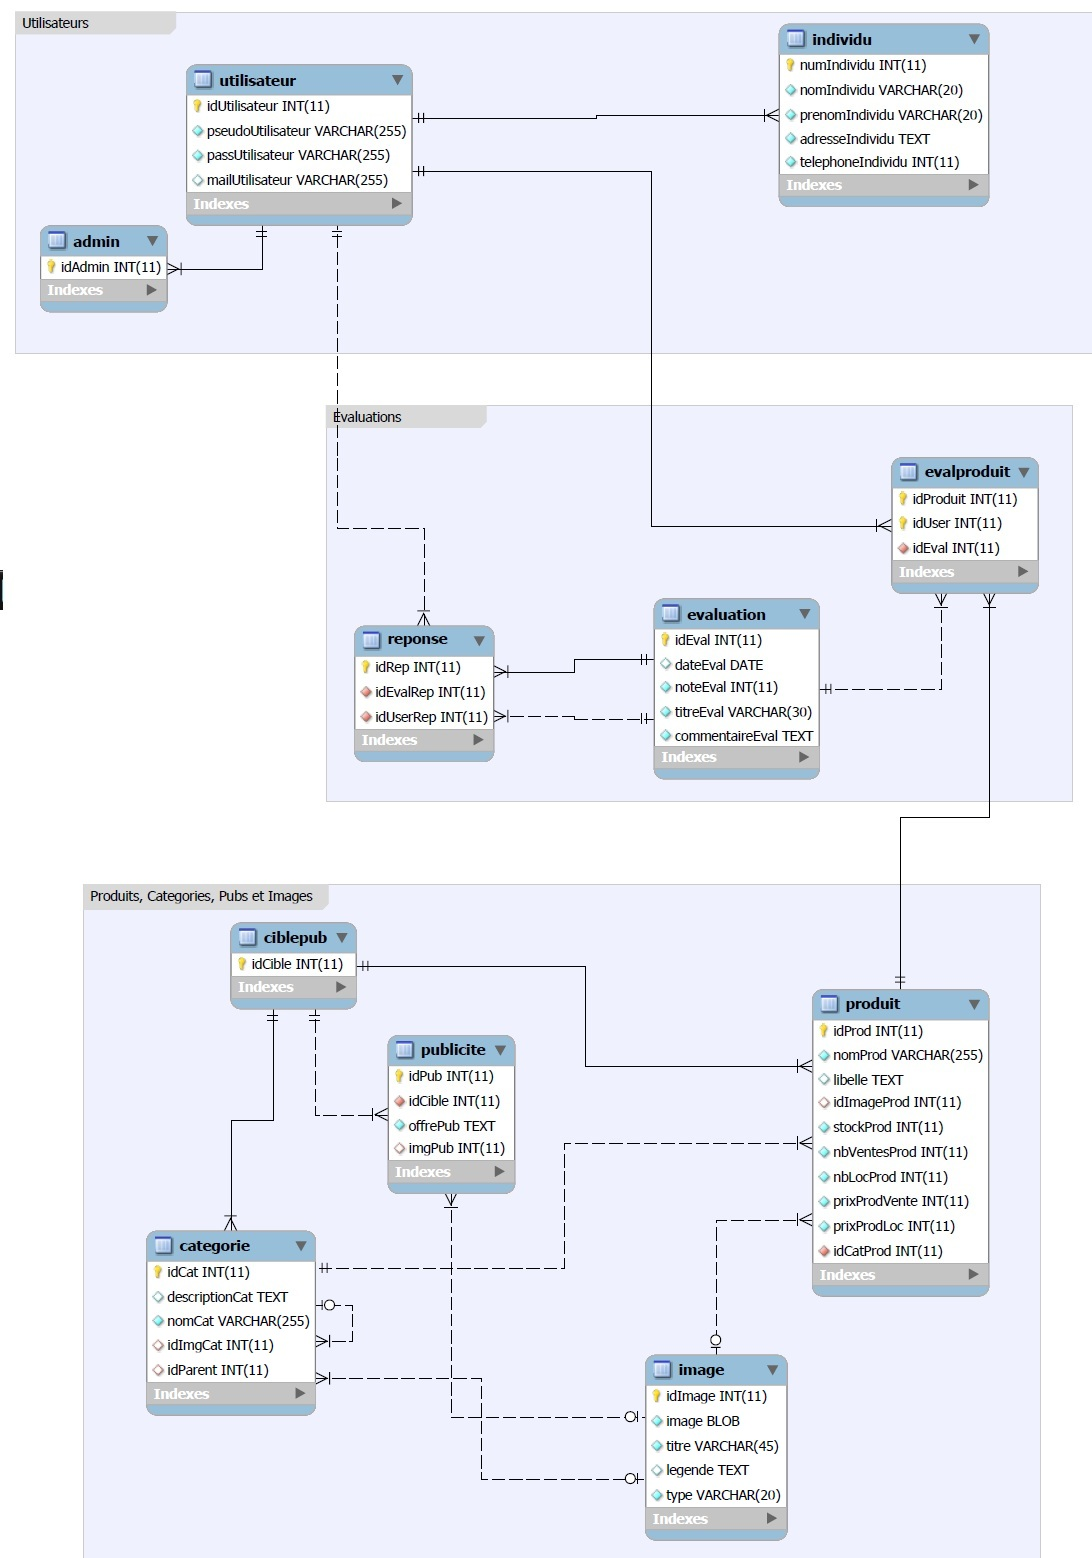
\includegraphics[scale=0.5]{dbob.jpg}	